\documentclass{exam}
\usepackage{tikz}
\usepackage{amssymb}
\usepackage{amsmath}
\title{CS113/DISCRETE MATHEMATICS-SPRING 2024}
\author{Worksheet 21}
\date{Topic: Introduction To Graphs}
\begin{document}
\maketitle

\begin{center}
\fbox{\fbox{\parbox{5.5in}{\centering Today, we'll delve into the concept of graphs, an essential tool for representing relationships between objects. Graphs consist of vertices connected by edges, allowing us to model various systems like social networks and transportation networks. Happy Learning!}}}
\end{center}

\vspace{5mm}
\makebox[0.75\textwidth]{Student's Name and ID:\enspace\hrulefill}

\vspace{5mm}
\makebox[0.75\textwidth]{Instructor’s name:\enspace\hrulefill}

\vspace{5mm}
\begin{questions}


\question 
Determine whether the graph shown has
directed or undirected edges, whether it has multiple edges,
and whether it has one or more loops. Use your answers to
determine the type of graph in Table 1 this graph is. Watch for diagrams on Projector's  screen.

\begin{parts}
\part 




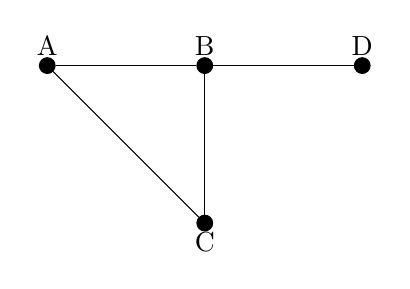
\begin{tikzpicture}
\node[circle, draw, fill, inner sep=2pt] (A) at (0,0) {};
\node[circle, draw, fill, inner sep=2pt] (B) at (2,0) {};
\node[circle, draw, fill, inner sep=2pt] (C) at (2,-2) {};
\node[circle, draw, fill, inner sep=2pt] (D) at (4,0) {};

\node[above] at (A) {A};
\node[above] at (B) {B};
\node[below] at (C) {C};
\node[above] at (D) {D};

\draw (A) -- (B);
\draw (A) -- (C);
\draw (B) -- (C);
\draw (B) -- (D);
\end{tikzpicture}
\vspace{3in}

\part 

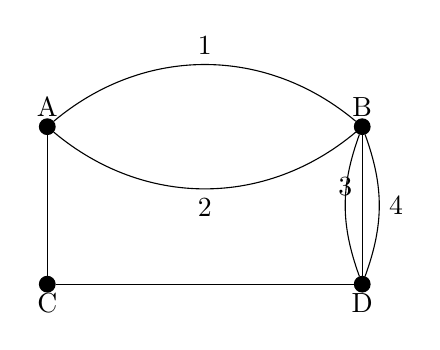
\begin{tikzpicture}
  \node[circle, draw, fill, inner sep=2pt] (A) at (0,0) {};
  \node[circle, draw, fill, inner sep=2pt] (B) at (4,0) {};
  \node[circle, draw, fill, inner sep=2pt] (C) at (0,-2) {};
  \node[circle, draw, fill, inner sep=2pt] (D) at (4,-2) {};

  \node[above] at (A) {A};
  \node[above] at (B) {B};
  \node[below] at (C) {C};
  \node[below] at (D) {D};

  \draw (A) to[out=40,in=140] node[above] {1} (B);
  \draw (A) to[out=-40,in=-140] node[below] {2} (B);
  \draw (B) to[out=250,in=110] node[above] {3} (D);
  \draw (B) to[out=290,in=70] node[right] {4} (D);
  \draw (B) to (D);
  \draw (A) -- (C);
  \draw (C) -- (D) ;
\end{tikzpicture}
\vspace{3in}

\part 
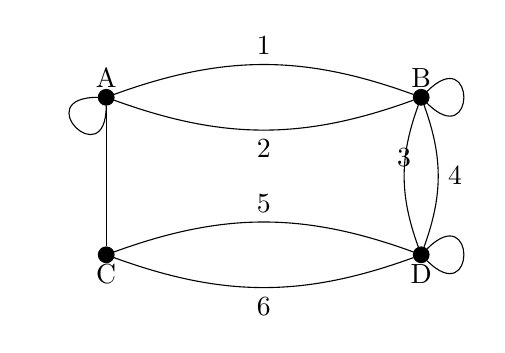
\begin{tikzpicture}
\node[circle, draw, fill, inner sep=2pt] (A) at (0,0) {};
\node[circle, draw, fill, inner sep=2pt] (B) at (4,0) {};
\node[circle, draw, fill, inner sep=2pt] (C) at (0,-2) {};
\node[circle, draw, fill, inner sep=2pt] (D) at (4,-2) {};

\node[above] at (A) {A};
\node[above] at (B) {B};
\node[below] at (C) {C};
\node[below] at (D) {D};

\draw (A) to [out=180,in=270,looseness=15] (A);
\draw (B) to [out=45,in=-45,looseness=15] (B);
\draw (D) to [out=45,in=-45,looseness=15] (D);
\draw (A) to[out=20,in=160] node[above] {1} (B);
\draw (A) to[out=-20,in=-160] node[below] {2} (B);
\draw (B) to[out=250,in=110] node[above] {3} (D);
\draw (B) to[out=290,in=70] node[right] {4} (D);
\draw (C) to[out=20,in=160] node[above] {5} (D);
\draw (C) to[out=-20,in=-160] node[below] {6} (D);
\draw (A) -- (C);
\end{tikzpicture}
\vspace{3in}

\part
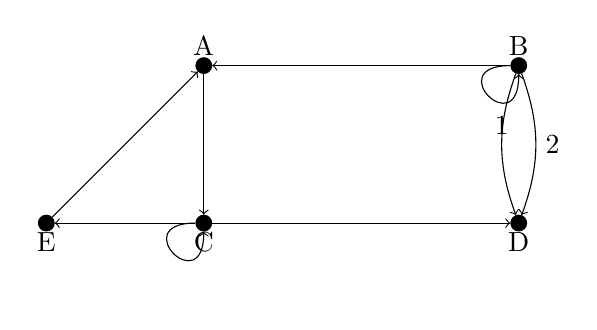
\begin{tikzpicture}
\node[circle, draw, fill, inner sep=2pt] (A) at (0,0) {};
\node[circle, draw, fill, inner sep=2pt] (B) at (4,0) {};
\node[circle, draw, fill, inner sep=2pt] (C) at (0,-2) {};
\node[circle, draw, fill, inner sep=2pt] (D) at (4,-2) {};
\node[circle, draw, fill, inner sep=2pt] (E) at (-2,-2) {};


\node[above] at (A) {A};
\node[above] at (B) {B};
\node[below] at (C) {C};
\node[below] at (D) {D};
\node[below] at (E) {E};
\draw[->] (E) -- (A);
\draw[->] (A) -- (C);
\draw[->] (C) -- (E);
\draw[->] (B) -- (A);
\draw[->] (C) -- (D);
\draw[->] (C) to [out=180,in=270,looseness=15] (C);
\draw[->] (B) to [out=180,in=270,looseness=15] (B);
\draw[->] (B) to[out=250,in=110] node[above] {1} (D);
\draw[->] (B) to[out=290,in=70] node[right] {2} (D);

\end{tikzpicture}

\vspace{3in}

\end{parts}
\question  Describe a graph model that represents traditional marriages between men and women. Does this graph have
any special properties?
\vspace{9in}


\question
Describe a graph model that represents whether each person at a party knows the name of each other person at the
party. Should the edges be directed or undirected? Should
multiple edges be allowed? Should loops be allowed?
\vspace{9in}

\question

Construct the call graph for a set of seven telephone
numbers 555-0011, 555-1221, 555-1333, 555-8888,
555-2222, 555-0091, and 555-1200 if there were three
calls from 555-0011 to 555-8888 and two calls from
555-8888 to 555-0011, two calls from 555-2222 to
555-0091, two calls from 555-1221 to each of the
other numbers, and one call from 555-1333 to each of
555-0011, 555-1221, and 555-1200.



\end{questions}
\end{document}